\section{Echo State Network}
\label{sc:esn}
Um die zuvor erwähnten Probleme der \textsc{RNN} zu umgehen, wurden als mögliche Lösung die \textsc{Echo State Networks} von H. Jäger vorgeschlagen \cite{jaeger2010}. Etwa zeitgleich wurde von W. Maas das Modell der \textit{Liquid State Machines} (\textsc{ESN}) vorgeschlagen. In diesem Modell steht der biologische Hintergrund im Fokus, doch sind die Ergebnisse denen der \textsc{Echo State Networks} sehr ähnlich \citep{Maass2011}. 

\subsection{Aufbau}
\label{sec:esn_structure}
Ein \textsc{ESN} ist eine Spezialform eines \textsc{RNN}s. Hierbei wird eine auf dem ersten Blick eigenartige Entscheidung getroffen: Während des gesamten Trainingsvorganges werden die Verbindungen der einzelnen Einheiten größtenteils nicht verändert. Es wird versucht durch das \textit{Echo} der vorherigen Signale, welche noch im Netzwerk gespeichert sind, diese Signale zu rekonstruieren - hieraus ergibt sich auch der Name \cite{lukoseviciusa2009}. Im Folgenden wird der Aufbau und anschließend die Funktionsweise eines solchen Netzwerkes nach \citep{jaeger2007} beschrieben.\\

Allgemein bildet das Netzwerk $E$ ein zeitliches Signal $\vec{u}(n) \in \mathbb{R}^{N_u}$  auf eine zeitlich variable Ausgabe $\vec{y}(n) \in \mathbb{R}^{N_y}$ für die Zeiten $n=1, ..., T$ ab. Zudem besitzt das System ein sogenanntes \textit{Reservoir} aus $N$ nicht-linearen Einheiten. Der innere Zustand des Netzwerkes wird durch diese Einheiten beschrieben und als $s(n) \in \mathbb{R}^{N}$ bezeichnet.\\

Die Verbindungen der inneren Einheiten untereinander werden durch die Gewichtsmatrix $\mathbf{W} \in \mathbb{R}^{N \times N}$ beschrieben. Das Eingangssignal wird zusammen mit einem \textit{Bias} $b_{in} \in \mathbb{R}$ durch die Matrix $\mathbf{W_{in}} \in \mathbb{R}^{N \times (N_u+1)}$ auf die inneren Einheiten weitergeleitet. Eine Rückkopplung zwischen Ausgabesignal und internen Einheiten wird durch die Matrix $\mathbf{W_{fb}} \in \mathbb{R}^{N \times N_y}$ ermöglicht. In Abbildung \ref{fig:esn_structure} ist der vollständige Struktur eines \textsc{ESN}s mit den Matrizen $\mathbf{W_{in}}, \mathbf{W}, \mathbf{W_{fb}}$ und $\mathbf{W_{out}}$ dargestellt.

\begin{figure}[h]
    \centering
    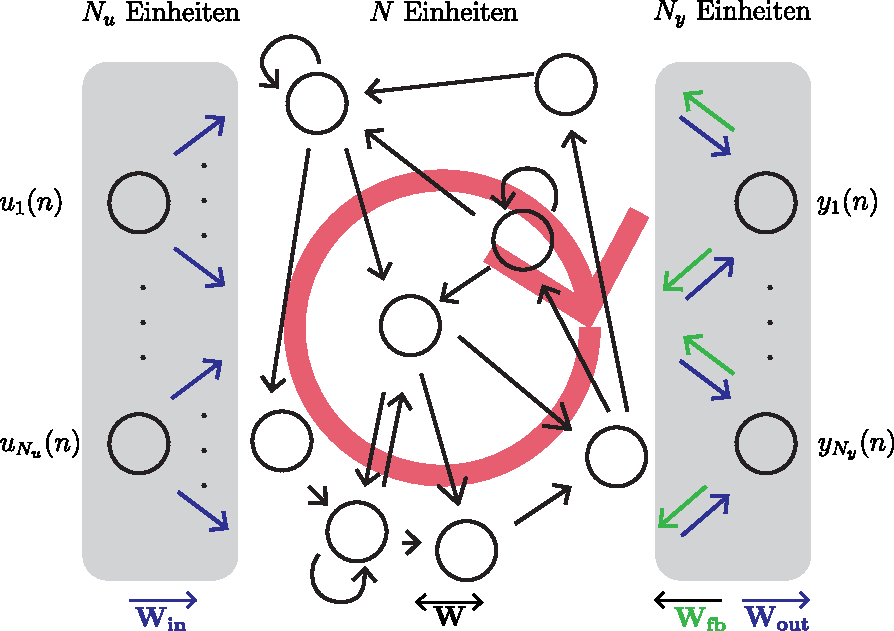
\includegraphics[width = 0.7 \textwidth]{figures/illustrations/esn_structure.pdf}
    \caption{Schematische Darstellung eines \textsc{ESN}. Von links nach rechts durchläuft das Eingangssignal $u(n)$ erst $N_u$ Eingangseinheiten, danach ein Reservoir mit $N$ Einheiten, bis schließlich die Ausgabe $y(n)$ mittels $N_y$ Ausgabeeinheiten gebildet wird. (nach \citep{jeagerTut2002, Ma2013}).}
    \label{fig:esn_structure}
\end{figure}


Die zeitliche Entwicklung der inneren Zustände kann, motiviert durch ein gewöhnliches Neuron, durch die Zustandsgleichung
\begin{align}
\vec{s}(n) = f_{in}\left( \mathbf{W_{in}} [b_{in}; \vec{u}(n)] + \mathbf{W} \vec{s}(n-1) \right).
\end{align}
bestimmt werden. Dabei ist $f_{in}$ eine beliebige (meistens \textit{sigmoid}-förmige) Transferfunktion, und $[\cdot\,;\,\cdot]$ das vertikale Aneinanderfügen von Vektoren beziehungsweise Matrizen bezeichnet. In dieser Arbeit wird die Tansferfunktion $f_{in} = \tanh(\cdot)$ genutzt.\\

Bessere Ergebnisse lassen sich durch das Abändern der Zustandsgleichung zu
\begin{align}
\label{eq:esn_stateeq}
\vec{s}(n) = (1 - \alpha) \cdot \vec{s}(n-1)  + \alpha \cdot f_{in}\left( \mathbf{W_{in}} [b_{in}; \vec{u}(n)] + \mathbf{W} \vec{s}(n-1) \right),
\end{align}
erreichen. Für diese Zustandsgleichung wurde das Modell eines \textit{Leaky Integrator Neurons} genutzt, wobei $\alpha \in (0,1]$ die Verlustrate beschreibt. Für $\alpha=1$ ergibt sich als Spezialfall ein gewöhnliches Neuron mit der oben beschriebenen Zustandsgleichung.\\

Da für manche Anwendungsfälle auch eine direkte Rückkopplung wünschenswert ist, kann das System noch um eine Ausgabe-Rückkopplung erweitert werden. Diese verbindet die Ausgabe erneut mit den inneren Einheiten durch die Matrix $\mathbf{W_{fb}} \in \mathbb{R}^{N \times N_y}$.
Somit ergibt sich 
\begin{align}
\label{eq:esn_stateeq_feedback}
\vec{s}(n) = (1 - \alpha) \cdot \vec{s}(n-1) + \alpha \cdot f_{in}\left( \mathbf{W_{in}} [b_{in}; \vec{u}(n)] + \mathbf{W} \vec{s}(n-1) + \mathbf{W_{fb}} \vec{y}(n) \right)
\end{align}
als Zustandsgleichung. Solche Rückkopplungen werden meistens nur benutzt um autonom arbeitenden Modelle zu erzeugen. Da dies für die Anwendungen in dieser Arbeit nicht gewünscht ist, wird im Folgenden die Rückkopplungsmatrix weggelassen.\\

Anhand der inneren Zustände lassen sich nun noch die sogenannten erweiterten inneren Zustände $x(n) = [b_{out}; \vec{s}(n); \vec{u}(n)] \in \mathbb{R}^{1 + N + N_u}$ definieren, wobei $b_{out}$ einen \textit{Bias} für die Ausgabe darstellt.\\

Aus diesen erweiterten inneren Zuständen kann nun die Ausgabe $\vec{y}(n)$ konstruiert werden. Dies kann entweder im Sinne einer Linearkombination durch die Ausgangsmatrix $\mathbf{W_{out}} \in \mathbb{R}^{ N_y \times (1 + N + N_u)}$ oder durch andere nicht lineare Regressionsalgorithmen wie beispielsweise einer \textsc{Support Vector Machine (SVM)} durchgeführt werden. Im Folgenden wird nur der Fall einer Linearkombination betrachtet, da sich für die anderen Methoden ein analoges Verfahren ergibt.
In diesem Fall berechnet sich die Ausgabe mittels
\begin{align}
\vec{y}(n) = f_{out} \left( \mathbf{W_{out}} \vec{x}(n) \right) = f_{out} \left(\mathbf{W_{out}} [b_{out}; \vec{s}(n); \vec{u}(n)] \right),
\end{align}
wobei $f_{out}$ die Transferfunktion der Ausgabe ist. Für diese kann in den meisten Fällen (so auch in dieser Arbeit) die Identität $f_{out}(x) = x$ genutzt werden.\\

Während die Matrix $\mathbf{W_{out}}$ durch den Trainingsvorgang bestimmt wird, werden die Matrizen $\mathbf{W_{in}}$ und $\mathbf{W}$ a priori generiert und festgelegt. Hierbei hat sich für das Generieren der Eingangsmatrix eine zufällige Anordnung von gleichförmig verteilten Gleitkommazahlen zwischen $-0.5$ und $0.5$ als geschickt herausgestellt. Falls ein Feedback gewünscht ist, also Gleichung (\ref{eq:esn_stateeq_feedback}) genutzt wird, wird $\mathbf{W_{fb}}$ gleichartig konstruiert. Die innere Matrix $\mathbf{W}$ wird ebenfalls zufällig generiert, doch soll diese zugleich dünnbesetzt sein. Zudem gibt es hierfür weitere Merkmale, die erfüllt sein sollen. Darauf wird in Abschnitt \ref{sc:esn_theory} genauer eingegangen.

\subsection{Theoretischer Hintergrund}
\label{sc:esn_theory}
Um die mathematischen Eigenschaften beschreiben zu können, sind zuerst zwei Definitionen nötig \cite{yildiz}.

\begin{definition}[Kompatibler Zustand]
Sei $E : S \times U \rightarrow S$ ein \textsc{ESN} für den Zustandsraum $S$ und den Raum $U$ des Eingangssignals mit der Zustandsgleichung $\vec{s}(n+1) = F \left( \vec{s}(n), \vec{u}(n+1) \right)$. Eine Folge von Zuständen $(\vec{s}(n))_n$ ist kompatibel mit der Eingangsfolge $(\vec{u}(n))_n$, wenn $\vec{s}(n+1) = F\left( \vec{s}(n), \vec{u}(n+1) \right), \forall n$ erfüllt ist.
\end{definition}

\begin{definition}[Echo State Eigenschaft (ESP)]
Ein \textsc{ESN} $E : S \times U \rightarrow S$ besitzt die \textit{Echo State Eigenschaft} genau dann wenn eine Nullfolge $(\delta(n))_{n \geq 0}$ existiert, sodass für alle Paare von Zustandsfolgen $(\vec{s}(n))_n, (\vec{s}\,'(n))_n$ die kompatibel mit der Eingangsfolge $(\vec{u}(n))_n$ sind gilt, dass $\forall n \geq 0 ||\vec{s}(n) - \vec{s}\,'(n)|| < \delta_n$
\end{definition} 
Das Vorliegen der \textit{ESP} bedeutet anschaulich, dass nachdem das Netzwerk lang genug betrieben worden ist, der Zustand nicht mehr von dem beliebig gewähltem Anfangszustand abhängt. Stattdessen wird ein für das Signal und Netzwerk charakteristischer Zustand angenommen. Diese Eigenschaft ist notwendig, damit das \textsc{ESN} Vorhersagen treffen kann \cite{jeagerTut2002}.\\

Nun stellt sich die Frage, wann ein Netzwerk diese Eigenschaft besitzt. Da die Gewichtsmatrix $\mathbf{W}$ die internen Verbindungen beschreibt und somit einen sehr starken Einfluss auf die Dynamik hat, ist anzunehmen, dass die Eigenschaft hauptsächlich durch die Gewichtsmatrix $\mathbf{W}$ bestimmt wird.\\

In den letzten Jahren sind drei verschiedene Kriterien für das Auftreten der \textit{ESP} aufgestellt worden. Chronologisch ist zuerst bekannt gewesen, dass für einen Spektralradius $\rho(\mathbf{W}) > 1$ die Eigenschaft nicht auftreten kann, sofern $\vec{u}_n = 0$ möglich ist \cite{jaeger2007, jaeger2010}. Hieraus ergab sich lange Zeit die falsche Annahme, dass für Systeme mit $\rho(\mathbf{W}) < 1$ die Eigenschaft stets garantiert ist. Wie allerdings gezeigt werden konnte, ist dies nicht der Fall \citep{yildiz}.\\

Darauffolgend ist die hinreichende Bedingung für die \textit{ESP}
\begin{align}
\label{eq:theory_old_requirement}
|1-\alpha(1-\sigma_{max}(\mathbf{W}))| < 1
\end{align}
aufgestellt worden. Eine Beweisskizze der Herleitung dieser Bedingung ist in Anhang \ref{sc:apx_math_stability_proof} zu finden.\\

Darauf basierend ist eine weitere hinreichende Bedingung
\begin{align}
\label{eq:theory_sufficient_requirement}
\rho(\alpha |\mathbf{W}|+(1-\alpha) \mathbf{I}) < 1
\end{align}
hergeleitet worden. Wobei als Betrag der Matrix hier das elementweise Betragsnehmen gemeint ist. Diese Bedingung ist weniger einschränkend als Gleichung (\ref{eq:theory_old_requirement}) \cite{yildiz}.\\


Weitergehend hat sich in Experimenten gezeigt, dass eine dünnbesetze Gewichtsmatrix $\mathbf{W}$ zu reicheren Dynamiken innerhalb des Reservoirs führen kann. Dabei werden in der Literatur oftmals mehr als $80\%$ der Einträge auf $0$ gesetzt \citep{jaeger2010}. Eine solche dünnbesetze Matrix bedeutet, dass nicht mehr jedes Neuron mit jedem anderen Neuron verbunden ist, sondern dass nur noch ein relativer Anteil $\epsilon$ dieser Verbindungen vorhanden ist. Da durch eine größere Anzahl an verschiedenen internen Dynamiken vielfältigere Funktionen besser approximiert werden können, kann die Vorhersagequalität durch einen Geringen $\epsilon$ Wert erhöht werden.\\

Darauf basierend kann nun eine Methode nach \cite{yildiz} angegeben werden, um die Gewichtsmatrix $\mathbf{W}$ zu konstruieren:

\singlespacing
\begin{enumerate}
	\item Generiere zufällige Matrix $\mathbf{W}$ mit $\mathbf{|W|} = \mathbf{W}$ bei der in jeder Zeile nur $\epsilon$ Einträge ungleich $0$ sind.
	\item Skaliere $\mathbf{W}$, sodass Gleichung (\ref{eq:theory_sufficient_requirement}) erfüllt ist.
	\item Wechsel zufällig das Vorzeichen von ungefähr der Hälfte aller Einträge.
\end{enumerate}
\onehalfspacing

Statt dieser Vorschrift wurde zuvor oftmals $\mathbf{W}$ zufällig generiert und anschließend nur $\rho(\mathbf{W})$ statt $\rho(|\mathbf{W}|)$ skaliert, was mit unter zu instabilen Systemen geführt hat. Da allerdings auch für Systeme mit einem Spektralradius $ > 1$ die \textit{ESP} beobachtet werden kann für nicht verschwindende Eingänge $\vec{u}_n$, ist es ratsam auch effektive Spektralradien jenseits $1$ auszuprobieren.\\

Zusätzlich zu diesen Eigenschaften wird die Dynamik des Reservoirs auch von dessen Größe $N$ bestimmt. Es kann gezeigt werden, dass die Gedächtnisleistung eines Reservoirs stark von dieser abhängt. Somit ist es ratsam für Aufgaben, die eine lange Gedächtnisleistung benötigen, ein großes und für Aufgaben, die nur ein Kurzzeitgedächtnis benötigten, ein kleines Reservoir zu benutzen. \citep{jeagerTut2002}. Bei einer zu kleine Wahl für $N$ kann das Reservoir nicht die volle Dynamik des eigentlichen Systems wiedergeben. Bei einer zu großen Wahl von $N$ kann das \textit{Overfitting} auftreten: Dabei generalisiert das \textsc{ESN} die tatsächliche Dynamik des Systems nicht stark genug, sodass zwar ein geringer Trainingsfehler aber ein deutlich höherer Testfehler erreicht wird \citep{jeagerTut2002}.

\improvement{Write something about runtime complexity?} 

\subsection{Trainingsvorgang}
Nachdem der Aufbau des Netzwerkes beschrieben ist, ergibt sich nun die Frage, wie der Trainingsvorgang durchgeführt wird.

Hierfür wird für die Zeiten $n=0, ..., T_0$ das \textsc{ESN} mit dem Signal $\vec{u}(n)$ betrieben, wobei $T_0$ die \textit{transiente Zeit} beschreibt. Hierdurch soll das System aus seinem zufällig gewähltem Anfangszustand in einen charakteristischen Zustand übergehen. Anschließend wird das System für Zeiten $n < T + T_0$ weiter betrieben und die erweiterten Zustände $\vec{x}(n)$ als Spalten in der \textit{Zustandsmatrix} $\mathbf{X} \in \mathbb{R}^{(1 + N_u + N) \times T}$ gesammelt. Analog dazu werden die gewünschten Ausgaben $\vec{y}(n)$ nach dem Anwenden der Inversen $f^{-1}_{out}$ der Ausgabe-Transferfunktion $f_{out}$ auch als Spalten in der \textit{Ausgabematrix} $Y \in \mathbb{R}^{N_y \times T}$ gesammelt.
Nun wird eine Lösung der Gleichung
\begin{align}
\mathbf{Y} = \mathbf{W_{out}} \mathbf{X}
\end{align}
für $\mathbf{W}_{out}$ gesucht. Hierfür stehen mehrere Verfahren zur Verfügung, von denen zwei prominente erwähnt sein sollen.
Zum einen kann die Lösung durch eine \textit{Tikhonov Regularisierung} erhalten werden. Dabei wird die Kostenfunktion 
\begin{align}
\sum_n ||\vec{y}(n) - \mathbf{W_{out}}\vec{x}(n)||^2 + \beta \cdot \sum_i ||\vec{W}_{out, i}||^2
\end{align}
minimiert, welche aus der Summe der Fehlerquadrate und einem Gewichtsterm $\beta \cdot \sum_i ||\vec{W}_{out, i}||^2$ besteht. Dabei steht $\vec{W}_{out, i}$ für die jeweils $i$-te Zeile der Gewichtsmatrix und $\beta$ ist die Regularisierungskonstante. Der Gewichtsterm sorgt dafür, dass die Lösung ausgewählt wird, bei der zum einen die Fehler im Trainingsvorgang möglichst gering sind, aber trotzdem die Gewichte nicht zu groß werden. Da große Gewichte ein Zeichen dafür sind, dass eine zu starke Anpassung an die Trainingsdaten vorliegt, kann also die Regularisierung den Effekt des \textit{Overfittings} unterdrücken. Das Verfahren
\begin{align}
\label{eq:tikhonov}
\mathbf{W}_{out} = \mathbf{Y} \mathbf{X}^T \left(\mathbf{X} \mathbf{X}^T + \beta I \right)^{-1}
\end{align}
ist sehr leistungsstark, aber auch teilweise numerisch instabil. Bei geeigneter Wahl von $\beta$ können die besten Ergebnisse hinsichtlich der Genauigkeit der Vorsage erzielt werden \cite{lukoseviciusa2009}. Deshalb wird in dieser Arbeit auch nur dieses Lösungsverfahren verwendet. Die weiteren Lösungsansätze für das Gleichungssystem sind nur aus Gründen der Vollständigkeit angegeben.\\

Zum anderen kann zur Lösung die \textit{Moore-Penrose-Pseudoinverse} $\mathbf{X}'$ genutzt werden, sodass für die Ausgabematrix
\begin{align}
\label{eq:pseudo_inverse}
\mathbf{W_{out}} = \mathbf{Y} \mathbf{X}'
\end{align}
folgt. Dieses Verfahren ist zwar sehr rechenaufwendig aber dafür numerisch stabil \cite{lukoseviciusa2009, jaeger2012}. Nichts desto trotz, kann allerdings auf Grund des Fehlens einer Regularisierung leicht der Effekt des \textit{Overfittings} auftreten. Auf Grund dessen wird es in dieser Arbeit nicht verwendet.\\

Um das \textit{Overfitting} bei der Verwendung der Psuedoinversen zu reduzieren, kann in der Zustandsgleichung (\ref{eq:esn_stateeq}) beziehungsweise (\ref{eq:esn_stateeq_feedback}) eine leichte normalverteilte Störung $\vec{\nu}(n)$ addiert werden. Falls die \textit{Tikhonov Regularisierung} zur Lösung verwendet wird, erhöht die Verwendung der zufälligen Störung die Stabilität der Vorhersage des System. Dieser Ansatz beruht auf Empirie, da eine mathematische Begründung hierfür noch nicht vollständig gelungen ist \citep{jaeger2010, lukoseviciusa2009}. Anschaulich lässt sich das Vorgehen dadurch motivieren, dass hierdurch künstliche Datenpunkte in der nähe der vorhandenen Trainingsdaten emuliert werden, und somit eine größere Vielfalt an Daten während der Trainingsphase beobachtet wird.\\

\begin{minipage}{\textwidth}
Zusammenfassend ergibt sich somit der folgende Funktionsablauf für die Anwendung eines \textsc{ESN}:

\singlespacing
\begin{enumerate}
	\item Zufälliges Generieren der Matrizen $\mathbf{W_{in}}, \mathbf{W_{fb}}$ und Konstruktion der Matrix $\mathbf{W}$ 
	\item Einspeisen des Signals $u(n)$ und Konstruktion der Zustandsmatrix $\mathbf{X}$ und der Ausgabematrix $\mathbf{Y}$ 
	\item Berechnung der Ausgabematrix $\mathbf{W_{out}}$
	\item Einspeisen des Signals $\vec{u}(n)$ für Vorhersagen des Signales $\vec{y}(n)$ für $n > T + T_0$
\end{enumerate}
\onehalfspacing
\end{minipage}

